%======================================================
%  DOCUMENTATION PIPELINE ECOLAB
%======================================================
\documentclass[11pt,a4paper]{report}

%--- Encodage & langue ---
\usepackage[utf8]{inputenc}
\usepackage[T1]{fontenc}
\usepackage[french]{babel}

%--- Mise en page ---
\usepackage[top=2cm, bottom=2cm, left=2cm, right=2cm]{geometry}
\usepackage{setspace}
\setstretch{1.15}

%--- Polices & couleurs ---
\usepackage{lmodern}
\usepackage[dvipsnames,svgnames,table]{xcolor}
% ─── Couleurs ───
\definecolor{vert}{RGB}{46, 139, 87}
\definecolor{vertfonce}{RGB}{31, 92, 58}
\definecolor{vertclair}{RGB}{240, 247, 240}
\definecolor{gristexte}{RGB}{85, 85, 85}
\definecolor{codebg}{RGB}{248, 248, 248}
\definecolor{codeleft}{RGB}{46, 139, 87}
\definecolor{seuilrouge}{HTML}{d73027}
\definecolor{seuilorange}{HTML}{fc8d59}
\definecolor{seuilgris}{HTML}{d9d9d9}
\definecolor{seuilvertclair}{HTML}{91cf60}
\definecolor{seuilvertfonce}{HTML}{1a9641}

%--- Graphiques & figures ---
\usepackage{graphicx}
\usepackage{float}
\usepackage{caption}
\usepackage{subcaption}
\usepackage{tikz}
\usetikzlibrary{shapes.geometric, arrows.meta, positioning, fit, backgrounds, calc}

%--- Tableaux ---
\usepackage{booktabs}
\usepackage{tabularx}
\usepackage{longtable}
\usepackage{array}
\usepackage{multirow}
\usepackage{colortbl}
% ─── Tableaux ───
\newcolumntype{L}[1]{>{\raggedright\arraybackslash}p{#1}}
\renewcommand{\arraystretch}{1.4}

%--- Listes & puces ---
\usepackage{enumitem}

%--- Liens & PDF ---
\usepackage[colorlinks=true, linkcolor=NavyBlue, citecolor=ForestGreen,
            urlcolor=RoyalBlue, bookmarks=true]{hyperref}
\usepackage{bookmark}

%--- Code source ---
\usepackage{listings}
\lstset{
  basicstyle=\ttfamily\small,
  keywordstyle=\color{NavyBlue}\bfseries,
  commentstyle=\color{gray}\itshape,
  stringstyle=\color{ForestGreen},
  breaklines=true,
  frame=single,
  rulecolor=\color{gray!40},
  backgroundcolor=\color{gray!5},
  numbers=left,
  numberstyle=\tiny\color{gray},
  numbersep=6pt,
  xleftmargin=12pt,
  captionpos=b
}
\lstdefinelanguage{Python3}{
  language=Python,
  morekeywords={True,False,None,async,await,yield,from,import,as,with,assert,lambda}
}

%--- Boîtes colorées ---
\usepackage[most]{tcolorbox}
\tcbuselibrary{skins,breakable}

\newtcolorbox{infobox}[2][]{
  colback=SkyBlue!10, colframe=RoyalBlue!70,
  title=#2, fonttitle=\bfseries\small,
  #1
}
\newtcolorbox{warnbox}[2][]{
  colback=Orange!10, colframe=Orange!80,
  title=#2, fonttitle=\bfseries\small,
  #1
}
\newtcolorbox{codebox}[2][]{
  colback=gray!5, colframe=gray!40,
  title=#2, fonttitle=\ttfamily\small,
  #1
}

%--- En-têtes & pieds de page ---
\usepackage{fancyhdr}
\pagestyle{fancy}
\fancyhf{}
\fancyhead[L]{\small\textit{Pipeline EcoLab v2}}
\fancyhead[R]{\small\textit{\leftmark}}
\fancyfoot[C]{\thepage}
\renewcommand{\headrulewidth}{0.4pt}

%--- Macros utiles ---
\newcommand{\code}[1]{\texttt{\small #1}}
\newcommand{\gpkg}{\textsc{GeoPackage}}
\newcommand{\cosia}{\textsc{COSIA}}
\newcommand{\bdtopo}{\textsc{BD TOPO}}
\newcommand{\scot}{\textsc{SCoT}}
\newcommand{\todo}[1]{\textcolor{red}{\textbf{[TODO: #1]}}}

%--- Couleurs de score ---
\definecolor{scoreQ1}{HTML}{1a7a2e}
\definecolor{scoreQ2}{HTML}{7ec850}
\definecolor{scoreQ3}{HTML}{f5e642}
\definecolor{scoreQ4}{HTML}{f5a623}
\definecolor{scoreQ5}{HTML}{d0021b}

%======================================================
\begin{document}

%--- Page de titre ---
\begin{titlepage}
  \centering
  \vspace*{2cm}
  {\Huge\bfseries Rapport EcoLab\par}
  \vspace{0.5em}
  {\Large\color{NavyBlue} Documentation technique complète\par}
  \vspace{2cm}
  \rule{\textwidth}{1pt}
  \vspace{1em}
  {\large
  De la modélisation thématique (BERTopic) \\[0.3em]
  à la cartographie interactive \\[0.3em]
  des scores de préservation du territoire du SCoT \par
  }
  \vspace{1em}
  \rule{\textwidth}{1pt}
  \vspace{2cm}
  \begin{tabular}{ll}
    \textbf{Auteur :}   & ALVES Enrique, PINA Ruben, FAGE Annaelle,\\
    ~ & MAITRET Charles, YOUNES Rayane \\[0.3em]
    \textbf{Version :}  & 2.0 \\[0.3em]
    \textbf{Date :}     & Mars 2026 \\[0.3em]
    \textbf{Territoire :} & SCoT Drôme Ardèche (D007, D026, D084) \\[0.3em]
    \textbf{Corpus :}   & $\approx$50\,000 articles de presse environnementale \\[0.3em]
   
  \end{tabular}
  \vfill
%  {\small Ce document décrit l'intégralité de la chaîne de traitement : scraping, modélisation BERTopic, scoring LLM, analyse géospatiale, export QGIS et application web interactive.}
\end{titlepage}

\tableofcontents
\clearpage

%======================================================

\chapter*{Introduction}

L'aménagement durable des territoires nécessite aujourd'hui des outils de diagnostic précis, capables de concilier les dynamiques de développement local et les impératifs de préservation de la biodiversité. C'est dans ce contexte que s'inscrit le projet EcoLab, conçu spécifiquement pour le périmètre du Schéma de Cohérence Territoriale (SCOT) Drôme-Ardèche. Ce rapport technique, achevé en mars 2026, détaille l'intégralité d'une chaîne de traitement innovante visant à évaluer et cartographier les pressions d'artificialisation et la richesse écologique de ce territoire.

\subsection*{Les objectifs de la démarche}

La finalité du projet EcoLab est de fournir aux décideurs et aux planificateurs un outil cartographique interactif et méthodologiquement robuste. Nos objectifs principaux sont de :

\begin{itemize}
    \item Identifier les zones à fort potentiel écologique pour y prioriser les actions de conservation.
    \item Orienter de manière stratégique les inventaires naturalistes sur le terrain.
    \item Argumenter de façon chiffrée les zonages de protection dans le cadre de la révision du SCOT et des Plans Locaux d'Urbanisme intercommunaux (PLUi).
    \item Constituer un socle de données reproductible et opposable pour les futures études d'impact environnemental.
\end{itemize}

\subsection*{Une approche hybride et multi-échelles}

Pour répondre à ces exigences complexes, notre méthodologie s'articule autour de deux axes de modélisation complémentaires :

\begin{enumerate}
    \item \textbf{Une analyse sémantique et spatiale à l'échelle de la parcelle (Chapitre 1) :} Nous avons déployé une pipeline combinant l'Intelligence Artificielle et les Systèmes d'Information Géographique (SIG). En analysant un corpus d'environ 50 000 articles de presse environnementale grâce à la modélisation thématique (BERTopic) et à un modèle de langage (Mistral via Ollama), nous avons extrait un "signal territorial". Croisé à parité (50/50) avec le contexte géographique de la BD TOPO, ce signal permet d'attribuer à chaque polygone d'occupation des sols (COSIA) un score d'artificialisation allant de -2 (protecteur) à +2 (favorable au développement).
    \item \textbf{Une modélisation statistique globale à l'échelle de l'IRIS (Chapitre 2) :} Pour compléter cette vue granulaire, nous avons construit un score continu de potentiel écologique allant de 0 à 100. Ce score repose sur une Analyse en Composantes Principales (ACP) qui synthétise 12 indicateurs environnementaux et de pression issus de trois bases de données de référence (CarHAB, BD Forêt V2 et COSIA).
\end{enumerate}

Ce document documente en toute transparence nos choix techniques et d'architecture, depuis le traitement initial des données jusqu'à l'export final sous QGIS et le développement de notre application web interactive.

\chapter{BERTopic}

\section{Introduction et vue d'ensemble}

\subsection{Objectif du projet}

La pipeline EcoLab vise à produire une \textbf{carte de score d'artificialisation} à l'échelle parcellaire sur le territoire du \scot{} (Drôme-Ardèche). Pour chaque polygone de la couche \cosia{}, un score compris entre $-2$ (très favorable à la nature) et $+2$ (très favorable à l'artificialisation) est calculé à partir de deux sources complémentaires :

\begin{enumerate}
  \item \textbf{Le signal presse} : des articles de presse environnementale sont analysés par un modèle de langage (Ollama / Mistral) et regroupés par thème via BERTopic. Chaque classe d'occupation du sol hérite du score moyen des thèmes qui lui sont associés.
  \item \textbf{Le contexte géographique} : les couches \bdtopo{} (parcs naturels, forêts publiques, zones de végétation, cours d'eau, barrages, éoliennes…) enrichissent le score via un croisement spatial.
\end{enumerate}

Le score final est une combinaison pondérée 50/50 des deux sources, et est visualisé via QGIS et une application web Streamlit/Leaflet.

\subsection{Vue d'ensemble de la pipeline}

\begin{figure}[H]
\centering
% \resizebox adapte l'image à la largeur de la page (\textwidth)
\resizebox{\textwidth}{!}{%
\begin{tikzpicture}[
  node distance=0.8cm and 0.5cm, % Espacement global réduit
  % minimum width légèrement réduit à 3.8cm
  box/.style={rectangle, rounded corners=4pt, draw, minimum width=3.8cm, minimum height=0.85cm, align=center, font=\small},
  data/.style={box, fill=SkyBlue!20, draw=RoyalBlue!60},
  proc/.style={box, fill=ForestGreen!15, draw=ForestGreen!60},
  outs/.style={box, fill=Orange!15, draw=Orange!60},
  arr/.style={-{Stealth[length=5pt]}, thick},
  grp/.style={draw=gray!40, dashed, rounded corners=6pt, inner sep=8pt}
]

% Données sources (Espacement réduit à 0.5cm)
\node[data] (arts) {Articles presse\\(7 sources CSV)};
\node[data, right=0.5cm of arts] (cosia) {Tuiles COSIA\\(3 dép., $\sim$15M poly.)};
\node[data, right=0.5cm of cosia] (bdtopo) {\bdtopo{} SHP\\(3 dép., 14 catégories)};
\node[data, right=0.5cm of bdtopo] (scot) {Masque SCoT\\(Parcelles\_SCOT.gpkg)};

% BERTopic
\node[proc, below=1.2cm of arts] (bertopic) {\textbf{BERTopic}\\Modélisation thématique};
\draw[arr] (arts) -- (bertopic);

% Étape 01
\node[proc, below=1cm of bertopic] (e01) {\textbf{Étape 01}\\Scoring Ollama/Mistral\\($-2$ à $+2$ par article)};
\draw[arr] (bertopic) -- (e01);

% Étape 03 (Rapproché de l'étape 01)
\node[proc, right=2cm of e01] (e03) {\textbf{Étape 03}\\Score COSIA géospatial\\(topic $\rightarrow$ classe)};
\draw[arr] (e01) -- (e03);
\draw[arr] (cosia) -- (e03);
\draw[arr] (scot) -- (e03);

% Étape 04
\node[proc, below=1cm of e03] (e04) {\textbf{Étape 04}\\Enrichissement \bdtopo{}\\(croisements spatiaux)};
\draw[arr] (e03) -- (e04);
\draw[arr] (bdtopo) -- (e04);

% Étape 05
\node[proc, below=1cm of e04] (e05) {\textbf{Étape 05}\\Export QGIS\\(quintiles + QML)};
\draw[arr] (e04) -- (e05);

% Étapes 06 (Rapproché de l'étape 05)
\node[proc, left=1cm of e05] (e06a) {\textbf{Étape 06a}\\Articles par parcelle\\(embeddings + LLM)};
\node[proc, below=0.8cm of e06a] (e06b) {\textbf{Étape 06b}\\Résumés \bdtopo{}\\(combinaisons)};
\node[proc, below=0.8cm of e06b] (e06c) {\textbf{Étape 06c}\\Injection GPKG\\(resume\_bdtopo)};
\draw[arr] (e05) -- (e06a);
\draw[arr] (e06a) -- (e06b);
\draw[arr] (e06b) -- (e06c);

% Output GPKG
\node[outs, below=1cm of e06c] (gpkg) {\textbf{GPKG Final}\\COSIA\_BD\_ecolab\_carte\_finale};
\draw[arr] (e06c) -- (gpkg);
\draw[arr] (e05) -- (gpkg);

% App web (Rapproché du GPKG)
\node[outs, right=1.5cm of gpkg] (app) {\textbf{Application web}\\Streamlit + Flask\\+ Leaflet.js};
\draw[arr] (gpkg) -- (app);

\end{tikzpicture}%
}
\caption{Schéma général de la pipeline EcoLab v2}
\end{figure}

\subsection{Volumes de données}

\begin{table}[H]
\centering
\begin{tabular}{lcl}
\toprule
\rowcolor{seuilgris!75}
\textbf{Composant} & \textbf{Volume} & \textbf{Remarques} \\
\midrule
Articles de presse & $\sim$50\,000 & Dédupliqués par URL \\
Topics BERTopic & 125+ & Variable selon le run \\
Classes COSIA & 15 & Fixes (nomenclature) \\
Catégories \bdtopo{} & 14 & Fixes (nomenclature) \\
Polygones COSIA (final) & $\sim$15 millions & 3 départements \\
GPKG final & 29,7 Go & Index R-Tree + 15 index SQL \\
Articles synthétiques & 29 & 15 COSIA + 14 \bdtopo{} \\
Combos \bdtopo{} avec résumé & $\sim$160 & Après seuil MIN\_POLYGONS \\
\bottomrule
\end{tabular}
\caption{Volumes de données de la pipeline}
\end{table}

%======================================================
\section{Modélisation thématique — BERTopic}

\subsection{Objectif et principe}

BERTopic est un modèle de \textit{topic modeling} neuronal qui exploite des embeddings de phrases (Sentence-BERT) pour regrouper des articles en thèmes cohérents. Il résout le problème clé suivant : \textbf{comment distinguer automatiquement les articles pertinents pour l'artificialisation des sols de ceux qui ne le sont pas ?}

Le workflow est :
\begin{enumerate}
  \item Encoder chaque article en vecteur dense (modèle multilingue)
  \item Réduire la dimension avec UMAP
  \item Clusteriser avec HDBSCAN
  \item Extraire les mots-clés de chaque cluster via TF-IDF de classe (c-TF-IDF)
  \item Attribuer un label humain-lisible à chaque topic
\end{enumerate}

\subsection{Entraînement (\code{bertopic\_train\_save.py})}

\subsubsection{Sources de données}

\begin{table}[H]
\centering
\begin{tabular}{lll}
\toprule
\rowcolor{seuilgris!75}
\textbf{Source} & \textbf{Fichier CSV} & \textbf{Type} \\
\midrule
Cerema & \code{cerema\_actualites.csv} & Actualités institutionnelles \\
Actu-Environnement & \code{actu\_environnement\_actualites.csv} & Presse spécialisée \\
Le Dauphiné & \code{ledauphine\_articles.csv} & Presse régionale \\
Le Monde & \code{lemonde\_articles.csv} & Presse nationale \\
Vert.eco & \code{vert\_eco\_articles.csv} & Presse écologie \\
\bottomrule
\end{tabular}
\caption{Sources d'articles utilisées}
\end{table}

\subsubsection{Paramètres du modèle}

\begin{lstlisting}[language=Python3, caption={Initialisation de BERTopic (bertopic\_train\_save.py)}]
# Modele d'embeddings multilingue
embedding_model = SentenceTransformer(
    "paraphrase-multilingual-MiniLM-L12-v2"
)

# Reduction de dimension
umap_model = UMAP(
    n_components=5,
    metric="cosine",
    random_state=42
)

# Clustering
hdbscan_model = HDBSCAN(
    min_cluster_size=20,
    prediction_data=True
)

# Vectorisation TF-IDF avec stopwords francais
vectorizer = CountVectorizer(
    ngram_range=(1, 2),
    stop_words=FRENCH_STOPWORDS  # ~45 mots
)

# Modele final
topic_model = BERTopic(
    embedding_model=embedding_model,
    umap_model=umap_model,
    hdbscan_model=hdbscan_model,
    vectorizer_model=vectorizer,
    nr_topics=50,
    min_topic_size=20
)
\end{lstlisting}

\subsubsection{Pré-traitement}

\begin{itemize}
  \item Mise en minuscules, normalisation des espaces
  \item Filtrage : documents $<$ 80 caractères supprimés
  \item Déduplication par URL
\end{itemize}

\subsubsection{Sorties}

\begin{itemize}
  \item \code{docs\_with\_topics.csv} — chaque article avec son topic et sa probabilité
  \item \code{topics\_info.csv} — métadonnées (topic ID, nom, top mots-clés, n documents)
  \item \code{bertopic\_model/} — modèle sérialisé (réutilisable)
\end{itemize}

\subsection{Séparation pertinent / non-pertinent}

Après l'entraînement, les topics sont examinés manuellement et mappés :

\begin{itemize}
  \item \textbf{Topics pertinents (125+)} : associés à au moins une classe COSIA ou catégorie \bdtopo{} dans \code{TOPIC\_COSIA\_MAP} et \code{TOPIC\_BDTOPO\_MAP} de \code{config\_v2.py}
  \item \textbf{Topic $-1$} : documents hors-thème (outliers HDBSCAN), ignorés
  \item \textbf{Topics non mappés} : thèmes généraux (politique, santé, sport…) sans lien territorial, ignorés dans le scoring
\end{itemize}

\begin{infobox}{Exemple de mapping topic → classe COSIA}
\small
\code{TOPIC\_COSIA\_MAP = \{}\\
\code{\ \ 3: ["Bâtiment", "Zone imperméable"],\ \ \# topic 3 = urbanisme}\\
\code{\ \ 7: ["Feuillu", "Conifère"],\ \ \ \ \ \ \ \ \# topic 7 = forêt}\\
\code{\ \ 12: ["Surface eau"],\ \ \ \ \ \ \ \ \ \ \ \ \ \ \ \# topic 12 = eau}\\
\code{\ \ ...\}}
\end{infobox}

\subsection{Visualisation (\code{bertopic\_code\_heatmap\_visu.py})}

Plusieurs graphiques sont générés pour explorer et valider le modèle :

\begin{enumerate}
  \item \textbf{Distribution} : histogramme (topic ID vs. nombre de documents)
  \item \textbf{Heatmap topic × source} : crosstab des counts par source de données
  \item \textbf{UMAP documents} : nuage de points 2D coloré par topic (outliers inclus)
  \item \textbf{UMAP topics} : centroïdes des topics avec taille proportionnelle au nombre de documents, labels TF-IDF affichés
  \item \textbf{Tableau récapitulatif} : export CSV (topic ID, nom, n\_docs)
\end{enumerate}

%======================================================
\section{Étape 01 — Scoring Ollama des articles}

\textbf{Script :} \code{01\_topic\_notes\_ollama\_v2.py}

\subsection{Objectif}

Pour chaque article du corpus (après assignation des topics par BERTopic), un score d'artificialisation est attribué par un LLM local (Mistral via Ollama) selon une grille de $-2$ à $+2$.

\subsection{Grille de scoring}

\begin{table}[H]
\centering
\begin{tabular}{>{\centering}p{1.5cm}p{10cm}}
\toprule
\rowcolor{seuilgris!75}
\textbf{Score} & \textbf{Signification} \\
\midrule
\rowcolor{scoreQ1!30} $-2$ & Résiste fortement à l'artificialisation (biodiversité, qualité de l'eau, espaces agricoles, zones protégées) \\
\rowcolor{scoreQ2!30} $-1$ & Dominante environnementale légère (mobilité douce, agriculture durable) \\
\rowcolor{scoreQ3!30} $0$  & Pas de lien territorial / neutre \\
\rowcolor{scoreQ4!30} $+1$ & Dominante développement légère (transports, réhabilitation de friches) \\
\rowcolor{scoreQ5!30} $+2$ & Favorise l'artificialisation (construction, infrastructure, immobilier) \\
\bottomrule
\end{tabular}
\caption{Grille de scoring Ollama}
\end{table}

\subsection{Architecture d'appel}

\begin{lstlisting}[language=Python3, caption={Appel Ollama avec parsing robuste du score}]
def ollama_call(prompt: str) -> str:
    """Appel POST a l'API Ollama locale (localhost:11434)."""
    payload = {
        "model": "mistral",
        "prompt": prompt,
        "stream": False
    }
    r = requests.post(OLLAMA_URL, json=payload, timeout=120)
    return r.json()["response"]

def parse_score(raw: str) -> int | None:
    """Extrait un entier entre -2 et +2 de la reponse LLM."""
    matches = re.findall(r"[-+]?\d", raw)
    for m in matches:
        v = int(m)
        if -2 <= v <= 2:
            return v
    return None
\end{lstlisting}

\subsection{Logique de reprise (checkpoint)}

Toutes les 50 articles, le fichier \code{docs\_scored\_v2.csv} est sauvegardé. Au prochain lancement, les articles déjà scorés sont sautés automatiquement — le traitement peut être interrompu et repris.

\subsection{Sorties}

\begin{itemize}
  \item \code{docs\_scored\_v2.csv} — tous les articles avec leur score LLM
  \item \code{topic\_score\_summary\_v2.csv} — score moyen/médian par topic (agrégation par \code{groupby("topic")})
\end{itemize}

%======================================================
\section{Étape 02 — Visualisation des topics}

\textbf{Script :} \code{02\_topic\_viz\_v2.py}

\subsection{Graphiques produits}

\begin{enumerate}
  \item \textbf{Distribution} : barres horizontales, nombre de documents par topic (trié croissant)
  \item \textbf{Scores} : barres horizontales, score moyen Ollama par topic avec codage couleur par quintile :
\end{enumerate}

\begin{table}[H]
\centering
\begin{tabular}{lll}
\toprule
\rowcolor{seuilgris!75}
\textbf{Couleur} & \textbf{Hex} & \textbf{Seuil} \\
\midrule
\cellcolor{seuilrouge!40} Rouge foncé & \textbf{\#d73027} & $\leq -0.5$ (très protecteur) \\
\cellcolor{seuilorange!40} Orange & \textbf{\#fc8d59} & $-0.5$ à $0$ (protecteur) \\
\cellcolor{seuilgris!50} Gris & \textbf{\#d9d9d9} & $0$ (neutre) \\
\cellcolor{seuilvertclair!40} Vert clair & \textbf{\#91cf60} & $0$ à $0.5$ (développement) \\
\cellcolor{seuilvertfonce!40} Vert foncé & \textbf{\#1a9641} & $\geq 0.5$ (très développement) \\
\bottomrule
\end{tabular}
\caption{Codage couleur des scores de topic (teintes pastel)}
\end{table}

%======================================================
\section{Étape 03 — Score géospatial COSIA}

\textbf{Script :} \code{03\_geospatial\_score\_cosia\_v2.py}

\subsection{Objectif}

Assigner un score d'artificialisation à chaque polygone de la couche \cosia{} en fonction de sa classe d'occupation du sol, via le mapping \code{TOPIC\_COSIA\_MAP}.

\subsection{Construction du score par classe}

Pour chaque classe COSIA :
$$
\text{score\_classe}(c) = \frac{1}{|T_c|} \sum_{t \in T_c} \text{score\_moyen}(t)
$$
où $T_c$ est l'ensemble des topics mappés à la classe $c$.

\subsection{Architecture de traitement parallèle}

\begin{lstlisting}[language=Python3, caption={Lecture parallèle des tuiles COSIA}]
# 6 workers I/O en parallele, traitement sequentiel
with ThreadPoolExecutor(max_workers=6) as executor:
    futures = {
        executor.submit(read_and_filter_tile, tile): tile
        for tile in all_tiles
    }
    for future in as_completed(futures):
        gdf = future.result()
        if gdf is not None and len(gdf) > 0:
            process_gdf(gdf)  # sequentiel pour la memoire
\end{lstlisting}

\subsection{Filtre géographique}

Plutôt qu'un découpage géométrique coûteux, un simple filtre par \textit{bounding box} (Lambert 93) est appliqué : les polygones dont le centroïde est en dehors du SCoT sont exclus. La bbox du SCoT est :
$$
(816\,777,\ 6\,340\,562,\ 914\,455,\ 6\,407\,100) \text{ [Lambert 93]}
$$

\subsection{Sorties}

\begin{itemize}
  \item \code{COSIA\_SCORE\_v2.gpkg} — polygones scorés (\textasciitilde{}15M lignes)
  \item \code{COSIA\_SCORE\_v2\_attrs.csv} — attributs seuls (sans géométrie)
\end{itemize}

%======================================================
\section{Étape 04 — Enrichissement BD TOPO}

\textbf{Script :} \code{04\_enrich\_cosia\_bdtopo\_v2.py}

\subsection{Objectif}

Enrichir chaque polygone COSIA avec son contexte géographique \bdtopo{} : 14 colonnes booléennes \code{bdtopo\_*} indiquent si le polygone intersecte une zone protégée, une forêt publique, un cours d'eau, etc.

\subsection{Les 14 catégories BD TOPO}

\begin{table}[H]
\centering
\begin{tabular}{lll}
\toprule
\rowcolor{seuilgris!75}
\textbf{Catégorie} & \textbf{Colonne} & \textbf{Type de zone} \\
\midrule
Natura 2000 & \code{bdtopo\_NATURA2000} & Protection européenne \\
Parc naturel régional & \code{bdtopo\_PARC\_PNR} & Protection nationale \\
Réserve naturelle & \code{bdtopo\_RESERVE\_NAT} & Protection nationale \\
Géoparc & \code{bdtopo\_GEOPARC} & Label UNESCO \\
Forêt publique & \code{bdtopo\_FORET\_PUBLIQUE} & ONF \\
Zone végétation forêt & \code{bdtopo\_ZONE\_VEG\_FORET} & Zone de végétation \\
Zone végétation vigne & \code{bdtopo\_ZONE\_VEG\_VIGNE} & Zone de végétation \\
Zone végétation verger & \code{bdtopo\_ZONE\_VEG\_VERGER} & Zone de végétation \\
Zone végétation lande & \code{bdtopo\_ZONE\_VEG\_LANDE} & Zone de végétation \\
Cours d'eau & \code{bdtopo\_COURS\_EAU} & Hydrographie \\
Surface en eau & \code{bdtopo\_SURFACE\_EAU} & Hydrographie \\
Barrage & \code{bdtopo\_BARRAGE} & Infrastructure \\
Éolienne & \code{bdtopo\_EOLIENNE} & Infrastructure \\
Cours d'eau nommé & \code{nom\_cours\_eau} & (texte, TOPONYME) \\
\bottomrule
\end{tabular}
\caption{Catégories BD TOPO et colonnes correspondantes}
\end{table}

\subsection{Score BD TOPO et score final}

Le score BD TOPO d'un polygone est la moyenne des scores des catégories actives :
$$
\text{score\_bdtopo}(p) = \frac{1}{|C_p|} \sum_{c \in C_p} \text{score\_classe\_bdtopo}(c)
$$

Le score final est une pondération 50/50 :
$$
\text{score\_final}(p) = \begin{cases}
  0.5 \times \text{score\_cosia}(p) + 0.5 \times \text{score\_bdtopo}(p) & \text{si } |C_p| > 0 \\
  \text{score\_cosia}(p) & \text{sinon}
\end{cases}
$$

\subsection{Optimisations}

\begin{itemize}
  \item \textbf{Index spatial R-Tree} construit une seule fois pour tout le GPKG COSIA
  \item \textbf{ZONE\_DE\_VEGETATION} (594\,000 entités) mise en cache après filtrage bbox initial
  \item Opérations vectorisées NumPy pour le calcul du score final
\end{itemize}

\subsection{Sorties}

\begin{itemize}
  \item \code{COSIA\_SCORE\_finale\_ecolab.gpkg} — polygones finaux avec toutes les colonnes
  \item \code{COSIA\_SCORE\_finale\_attrs.csv} — attributs seuls
\end{itemize}

%======================================================
\section{Étape 05 — Export QGIS}

\textbf{Script :} \code{05\_export\_qgis\_v2.py}

\subsection{Quintiles et couleurs}

Le score final est discrétisé en 5 classes par quintiles (20\%, 40\%, 60\%, 80\%) :

\begin{table}[H]
\centering
\begin{tabular}{llll}
\toprule
\rowcolor{seuilgris!75}
\textbf{Quintile} & \textbf{Couleur} & \textbf{Hex} & \textbf{Signification} \\
\midrule
\rowcolor{scoreQ1!20} Q1 (0–20\%) & Vert foncé & \code{\#1a7a2e} & Très protecteur \\
\rowcolor{scoreQ2!20} Q2 (20–40\%) & Vert clair & \code{\#7ec850} & Protecteur \\
\rowcolor{scoreQ3!20} Q3 (40–60\%) & Jaune & \code{\#f5e642} & Neutre/mixte \\
\rowcolor{scoreQ4!20} Q4 (60–80\%) & Orange & \code{\#f5a623} & Développement \\
\rowcolor{scoreQ5!20} Q5 (80–100\%) & Rouge & \code{\#d0021b} & Très développement \\
\bottomrule
\end{tabular}
\caption{Quintiles et palette de couleurs}
\end{table}

\subsection{Fichier QML}

Un fichier de style \code{.qml} est généré automatiquement avec les intervalles de quintiles, de sorte que QGIS charge le style dès l'ouverture du \gpkg{}.

\subsection{Grille de tuiles 1km × 1km}

En plus des polygones individuels, une grille de tuiles d'1 km² est calculée avec le score moyen pondéré par surface :
$$
\text{score\_tuile} = \frac{\sum_i \text{score}_i \times \text{aire}_i}{\sum_i \text{aire}_i}
$$

\subsection{Sorties}

\begin{itemize}
  \item \code{COSIA\_BD\_ecolab\_carte\_finale.gpkg} — \gpkg{} final (renommage sans copie)
  \item \code{COSIA\_BD\_ecolab\_carte\_finale.qml} — style QGIS auto-chargé
  \item Couche \code{TUILES\_SCORE} ajoutée au même \gpkg{}
\end{itemize}

%======================================================
\section{Étape 06a — Articles par parcelle}

\textbf{Script :} \code{06\_articles\_par\_parcelle\_v2.py}

\subsection{Objectif}

Associer 3 articles de presse pertinents à chaque classe COSIA et catégorie \bdtopo{}, via une recherche sémantique en deux temps.

\subsection{Workflow en 2 temps}

\begin{enumerate}
  \item \textbf{Recherche par embeddings (cosine similarity)} : Pour chaque label (classe/catégorie), un article synthétique de référence est encodé, puis les 15 articles les plus proches du corpus sont récupérés.
  \item \textbf{Scoring LLM} : Ollama/Mistral note chaque candidat de 0.0 à 1.0 pour sa pertinence. Les 3 meilleurs sont conservés.
\end{enumerate}

\subsection{Articles synthétiques}

Pour chaque label, un article de référence de 300–500 mots est rédigé manuellement, mentionnant explicitement le contexte du SCoT Drôme-Ardèche. Ceci guide la recherche sémantique vers des articles localement pertinents.

\subsection{Cache d'embeddings}

\begin{lstlisting}[language=Python3, caption={Système de cache d'embeddings}]
# Sauvegarde
np.save("articles_embeddings_cache.npy", embeddings_array)
pd.DataFrame({"url": urls}).to_csv("articles_embeddings_index.csv")

# Chargement (si cache existant)
if cache_exists:
    embeddings = np.load("articles_embeddings_cache.npy")
    urls = pd.read_csv("articles_embeddings_index.csv")["url"].tolist()
\end{lstlisting}

\subsection{Résumé COSIA par Ollama}

Pour chaque classe COSIA, un résumé de 3–5 phrases est généré par Mistral à partir des 3 articles retenus. Ce résumé est stocké dans \code{COSIA\_articles\_par\_classe.csv}.

\subsection{Sorties}

\begin{itemize}
  \item \code{COSIA\_articles\_par\_classe.csv} — 15 lignes (une par classe), avec 3 URLs + titres COSIA, 6 URLs + titres contexte, résumé
  \item \code{COSIA\_BD\_ecolab\_articles.qml} — Map Tips QGIS (HTML avec liens cliquables)
\end{itemize}

%======================================================
\section{Étape 06b — Résumés BD TOPO}

\textbf{Script :} \code{06b\_resume\_bdtopo.py}

\subsection{Objectif}

Générer un résumé textuel pour chaque combinaison unique de catégories \bdtopo{} présente dans le \gpkg{}. Par exemple, un polygone situé à la fois en forêt publique et en Natura 2000 reçoit un résumé spécifique à ce contexte.

\subsection{Clé de combinaison}

La clé est une liste triée et séparée par \code{|} des catégories actives :
\begin{center}
\code{"FORET\_PUBLIQUE|NATURA2000|ZONE\_VEG\_FORET"}
\end{center}

\subsection{Seuil et filtrage}

Seules les combinaisons comptant au moins \code{MIN\_POLYGONS} polygones reçoivent un résumé (évite les résumés pour des combinaisons anecdotiques). Ce seuil a été baissé lors du second run pour couvrir des combinaisons rares comme \code{EOLIENNE|FORET\_PUBLIQUE|ZONE\_VEG\_FORET}.

\subsection{Sorties}

\begin{itemize}
  \item \code{BDTOPO\_resume\_par\_combo.csv} — 160 lignes : \code{combo\_key}, \code{n\_polygones}, \code{resume\_bdtopo}
\end{itemize}

%======================================================
\section{Étape 06c — Injection des résumés dans le GPKG}

\textbf{Script :} \code{06c\_inject\_resume\_bdtopo.py}

\subsection{Objectif}

Injecter la colonne \code{resume\_bdtopo} directement dans la table SQLite du \gpkg{} pour éviter une jointure à l'exécution (plus rapide pour QGIS et l'application web).

\subsection{Optimisations SQLite}

\begin{lstlisting}[language=Python3, caption={Pragmas SQLite pour writes rapides}]
conn.execute("PRAGMA journal_mode=MEMORY")  # journal en RAM
conn.execute("PRAGMA synchronous=OFF")      # pas de fsync
conn.execute("PRAGMA cache_size=100000")    # 100K pages en cache
\end{lstlisting}

\subsection{Logique de mise à jour}

Pour chaque combinaison unique :
\begin{lstlisting}[language=Python3, caption={UPDATE ciblé par combo BD TOPO}]
# Construction de la clause WHERE
where_parts = []
for cat in ALL_BDTOPO_CATS:
    val = 1 if cat in active_cats else 0
    where_parts.append(f"bdtopo_{cat} = {val}")

sql = f"""
    UPDATE COSIA_SCORE_finale
    SET resume_bdtopo = ?
    WHERE {' AND '.join(where_parts)}
"""
conn.execute(sql, (resume_text,))
\end{lstlisting}

%======================================================
\section{Application web interactive}

\textbf{Script :} \code{app\_carte2.py}

\subsection{Architecture technique}

L'application combine trois couches :

\begin{figure}[H]
\centering
\begin{tikzpicture}[
  node distance=1cm,
  layer/.style={rectangle, rounded corners=6pt, draw, minimum width=9cm, minimum height=1.2cm, align=center, font=\small},
  arr/.style={-{Stealth[length=5pt]}, thick}
]
\node[layer, fill=RoyalBlue!20, draw=RoyalBlue] (front) {\textbf{Frontend — Leaflet.js (JavaScript)}\\ Rendu cartographique, pan/zoom, sélection de parcelle};
\node[layer, fill=ForestGreen!15, draw=ForestGreen, below=0.7cm of front] (mid) {\textbf{Mid-tier — Flask (Python, port 5050)}\\ API REST : GeoJSON par bbox, détail par FID, filtres};
\node[layer, fill=Orange!15, draw=Orange, below=0.7cm of mid] (back) {\textbf{Backend — SQLite3 + Index R-Tree}\\ GPKG 29.7 Go, 15M polygones, 15 index SQL};
\node[layer, fill=Purple!10, draw=Purple!60, left=0.3cm of front, minimum width=3cm, xshift=-2.5cm] (st) {\textbf{Streamlit}\\ Sidebar filtres\\ Panel détail};

\draw[arr] (front) -- (mid) node[midway, right] {\small HTTP};
\draw[arr] (mid) -- (back) node[midway, right] {\small SQLite};
\draw[arr, <->] (st) -- (front) node[midway, above] {\small iframe};
\end{tikzpicture}
\caption{Architecture de l'application web}
\end{figure}

\subsection{Flask — Routes API}

\begin{table}[H]
\centering
\begin{tabular}{ccc}
\toprule
\rowcolor{seuilgris!75}
\textbf{Route} & \textbf{Méthode} & \textbf{Rôle} \\
\midrule
\code{/api/features} & GET & GeoJSON des polygones dans la bbox courante \\
\code{/api/detail/<fid>} & GET & Tous les attributs d'un polygone (articles, scores…) \\
\code{/api/filter\_bbox} & GET & Bbox de l'ensemble des résultats filtrés \\
\code{/api/select/<fid>} & GET & Stocker le FID sélectionné en session \\
\bottomrule
\end{tabular}
\caption{Routes de l'API Flask}
\end{table}

\subsection{Filtre et chargement}

\begin{lstlisting}[language=Python3, caption={Requête SQL avec filtres dynamiques (api\_features)}]
conditions = ["1=1"]
params = []

# Filtre par classes COSIA
if classes_filter:
    placeholders = ",".join("?" * len(classes_filter))
    conditions.append(f"classe IN ({placeholders})")
    params.extend(classes_filter)

# Filtres BD TOPO (AND logique)
for cat in bdtopo_filter:
    conditions.append(f"bdtopo_{cat} = 1")

# Filtre bbox viewport
conditions.append("""
    (minx <= ? AND maxx >= ? AND miny <= ? AND maxy >= ?)
""")
params.extend([xmax_l93, xmin_l93, ymax_l93, ymin_l93])

sql = f"""
    SELECT fid, geom, classe, score_cosia
    FROM COSIA_SCORE_finale
    WHERE {' AND '.join(conditions)}
    LIMIT 5000
"""
\end{lstlisting}

\subsection{Système de cache des bbox}

Au démarrage de l'application, un thread de fond calcule et met en cache les \textit{bounding boxes} de chaque combinaison filtre :

\begin{lstlisting}[language=Python3, caption={Pré-calcul de la bbox par classe (background thread)}]
sql = """
    SELECT classe,
           MIN(minx) as xmin, MAX(maxx) as xmax,
           MIN(miny) as ymin, MAX(maxy) as ymax
    FROM COSIA_SCORE_finale
    GROUP BY classe
"""
# Resultat sauvegarde dans bbox_cache.json
# → zoom automatique instantane au filtrage suivant
\end{lstlisting}

\subsection{Sidebar Streamlit — Filtres}

\begin{figure}[H]
\centering
\begin{tikzpicture}[
  box/.style={rectangle, rounded corners=3pt, draw=gray!60, fill=white, minimum width=5cm, minimum height=0.5cm, font=\small, align=center},
  section/.style={rectangle, rounded corners=3pt, fill=NavyBlue!10, draw=NavyBlue!40, minimum width=5cm, minimum height=0.4cm, font=\small\bfseries, align=center}
]
\node[section] (s1) {Classes COSIA};
\node[box, below=0.1cm of s1] (c1) {Bâtiment};
\node[box, below=0.05cm of c1] (c2) {Zone imperméable};
\node[box, below=0.05cm of c2] (c3) {Surface eau};
\node[box, below=0.05cm of c3] (c4) {... (15 classes)};
\node[section, below=0.3cm of c4] (s2) {Contexte BD TOPO};
\node[box, below=0.1cm of s2] (b1) {Natura 2000};
\node[box, below=0.05cm of b1] (b2) {Parc naturel régional};
\node[box, below=0.05cm of b2] (b3) {... (14 catégories)};
\node[box, below=0.4cm of b3, fill=ForestGreen!15, draw=ForestGreen] (btn) {\textbf{Zoom sur sélection}};
\end{tikzpicture}
\caption{Sidebar Streamlit avec filtres}
\end{figure}

\subsection{Panel de détail parcelle}

Quand l'utilisateur clique sur une parcelle sur la carte :

\begin{enumerate}
  \item Leaflet envoie le FID à Flask (\code{/api/select/<fid>})
  \item Streamlit interroge \code{/api/detail/<fid>} (polling toutes les 2s)
  \item Le panel affiche :
    \begin{itemize}
      \item \textbf{Score global} avec jauge colorée
      \item Score COSIA / Score \bdtopo{} séparément
      \item \textbf{Badges} des catégories \bdtopo{} actives
      \item \textbf{Articles COSIA} (3 liens cliquables) + résumé Mistral
      \item \textbf{Articles contexte} (3–6 liens) pour le contexte \bdtopo{}
      \item \textbf{Résumé \bdtopo{}} généré par Ollama pour la combinaison
    \end{itemize}
\end{enumerate}

\subsection{Carte Leaflet}

\begin{lstlisting}[language=Python3, caption={Seuils de score et couleurs (app\_carte2.py)}]
# Seuils quantiles du GPKG final
SCORE_THRESHOLDS = [-0.531, -0.465, -0.396, -0.297]

# Palette de couleurs
SCORE_COLORS = ["#1a7a2e", "#7ec850", "#f5e642", "#f5a623", "#d0021b"]

# Rectangle SCoT (WGS84) affiche en tirets bleus
SCOT_BOUNDS = [[44.154, 4.460], [44.730, 5.709]]
L.rectangle(SCOT_BOUNDS, {color:'#1976D2', dashArray:'8 5', weight:2})
\end{lstlisting}

\textbf{Threshold de zoom} : les polygones individuels ne se chargent qu'à partir du zoom 13 (environ commune), pour éviter de saturer le navigateur.

\subsection{Performances}

\begin{table}[H]
\centering
\begin{tabular}{lc}
\toprule
\rowcolor{seuilgris!75}
\textbf{Opération} & \textbf{Temps typique} \\
\midrule
Requête bbox + GeoJSON (5000 poly.) & $<$ 200 ms \\
Requête détail (1 parcelle) & $<$ 50 ms \\
Calcul bbox filtre (cache chaud) & $<$ 10 ms \\
Calcul bbox filtre (sans cache) & $\sim$ 2–5 s \\
Démarrage Flask + index warmup & $\sim$ 5 s \\
\bottomrule
\end{tabular}
\caption{Performances de l'application web}
\end{table}

%======================================================
\section{Index SQLite et optimisations}

\textbf{Script :} \code{create\_indexes.py}

\subsection{Index créés}

15 index SQLite sont créés sur la table \code{COSIA\_SCORE\_finale} pour accélérer les filtres :

\begin{lstlisting}[language=Python3, caption={Création des index SQLite}]
indexes = [
    ("idx_classe",          "classe"),
    ("idx_bdtopo_NATURA2000", "bdtopo_NATURA2000"),
    ("idx_bdtopo_PARC_PNR",   "bdtopo_PARC_PNR"),
    # ... 12 autres categories bdtopo
]

for idx_name, col_name in indexes:
    conn.execute(f"""
        CREATE INDEX IF NOT EXISTS {idx_name}
        ON COSIA_SCORE_finale ({col_name})
    """)
\end{lstlisting}

\begin{warnbox}{Temps de création}
Chaque index prend $\sim$40 minutes sur le \gpkg{} de 29.7 Go (15M lignes). Au total : $\sim$10 heures. À n'effectuer qu'une seule fois.
\end{warnbox}

%======================================================
\section{Configuration centrale}

\textbf{Fichier :} \code{config\_v2.py}

Toute la pipeline est configurée depuis un seul fichier. Les paramètres principaux :

\begin{lstlisting}[language=Python3, caption={Extraits de config\_v2.py}]
# Chemins
BASE_DIR = Path(__file__).parent
OUT_DIR  = BASE_DIR / "outputs"
GEO_DIR  = OUT_DIR / "geo"

# Ollama
OLLAMA_URL     = "http://localhost:11434/api/generate"
OLLAMA_MODEL   = "mistral"
OLLAMA_TIMEOUT = 120
SLEEP_BETWEEN  = 0.3  # secondes entre les appels

# Departements
COSIA_DEPTS = ["D007", "D026", "D084"]
BDTOPO_DEPTS = ["D007", "D026", "D084"]

# Bbox SCoT [Lambert 93]
SCOT_BBOX = (816777, 6340562, 914455, 6407100)

# Mapping topic -> classes COSIA (125+ topics)
TOPIC_COSIA_MAP = {
    3:  ["Batiment", "Zone impermeable"],
    7:  ["Feuillu", "Conifere"],
    12: ["Surface eau"],
    ...
}

# Mapping topic -> categories BD TOPO (40+ topics)
TOPIC_BDTOPO_MAP = {
    5:  ["NATURA2000"],
    9:  ["FORET_PUBLIQUE", "ZONE_VEG_FORET"],
    ...
}
\end{lstlisting}

%======================================================
\section{Lancement de la pipeline}

\subsection{Prérequis}

\begin{itemize}
  \item Python 3.10+, GDAL/GeoPandas, PyProj, Sentence-Transformers, BERTopic
  \item Ollama installé localement avec le modèle Mistral (\code{ollama pull mistral})
  \item QGIS 3.40+ pour la visualisation
  \item Streamlit (\code{pip install streamlit flask}) pour l'application web
\end{itemize}

\subsection{Ordre d'exécution}

\begin{table}[H]
\centering
\begin{tabular}{cll}
\toprule
\rowcolor{seuilgris!75}
\textbf{Ordre} & \textbf{Script} & \textbf{Durée approx.} \\
\midrule
0 & \code{bertopic\_train\_save.py} & 30–60 min \\
1 & \code{01\_topic\_notes\_ollama\_v2.py} & 3–8h (50K articles) \\
2 & \code{02\_topic\_viz\_v2.py} & 1–2 min \\
3 & \code{03\_geospatial\_score\_cosia\_v2.py} & 30 min \\
4 & \code{04\_enrich\_cosia\_bdtopo\_v2.py} & 45–90 min \\
5 & \code{05\_export\_qgis\_v2.py} & 10–20 min \\
6a & \code{06\_articles\_par\_parcelle\_v2.py} & 30–60 min \\
6b & \code{06b\_resume\_bdtopo.py} & 30–60 min \\
6c & \code{06c\_inject\_resume\_bdtopo.py} & 10–30 min \\
— & \code{create\_indexes.py} & $\sim$10h (une fois) \\
\bottomrule
\end{tabular}
\caption{Ordre et durée d'exécution des scripts}
\end{table}

\subsection{Lancement de l'application web}

\begin{lstlisting}[language=bash, caption={Démarrage de l'application Streamlit}]
cd pipeline_v2
streamlit run app_carte2.py
# Interface disponible sur http://localhost:8501
# API Flask sur http://localhost:5050
\end{lstlisting}

%======================================================
\section{Flux de données complet}

\begin{figure}[H]
\centering
\begin{tikzpicture}[
  node distance=0.5cm and 0.3cm,
  file/.style={rectangle, rounded corners=2pt, draw=gray, fill=gray!10, font=\tiny, minimum height=0.45cm, text width=3.2cm, align=center},
  step/.style={rectangle, rounded corners=4pt, draw=NavyBlue!60, fill=NavyBlue!10, font=\small\bfseries, minimum height=0.7cm, text width=3.8cm, align=center},
  arr/.style={-{Stealth[length=4pt]}, gray},
  thickarr/.style={-{Stealth[length=5pt]}, NavyBlue, thick}
]

\node[file] (f0) {docs\_with\_topics.csv};
\node[step, below=0.3cm of f0] (s01) {01 — Scoring Ollama};
\node[file, below=0.3cm of s01] (f1) {docs\_scored\_v2.csv\\topic\_score\_summary\_v2.csv};
\node[step, below=0.3cm of f1] (s03) {03 — Score COSIA géospatial};
\node[file, below=0.3cm of s03] (f2) {COSIA\_SCORE\_v2.gpkg};
\node[step, below=0.3cm of f2] (s04) {04 — Enrichissement BD TOPO};
\node[file, below=0.3cm of s04] (f3) {COSIA\_SCORE\_finale\_ecolab.gpkg};
\node[step, below=0.3cm of f3] (s05) {05 — Export QGIS};
\node[file, below=0.3cm of s05] (f4) {COSIA\_BD\_ecolab\_carte\_finale.gpkg\\ + .qml};
\node[step, below=0.3cm of f4] (s06a) {06a — Articles par classe};
\node[file, below=0.3cm of s06a] (f5) {COSIA\_articles\_par\_classe.csv};
\node[step, below=0.3cm of f5] (s06b) {06b — Résumés BD TOPO combos};
\node[file, below=0.3cm of s06b] (f6) {BDTOPO\_resume\_par\_combo.csv};
\node[step, below=0.3cm of f6] (s06c) {06c — Injection GPKG};
\node[file, below=0.3cm of s06c] (f7) {\textbf{GPKG FINAL}\\(+ resume\_bdtopo)};

\draw[thickarr] (f0) -- (s01);
\draw[thickarr] (s01) -- (f1);
\draw[thickarr] (f1) -- (s03);
\draw[thickarr] (s03) -- (f2);
\draw[thickarr] (f2) -- (s04);
\draw[thickarr] (s04) -- (f3);
\draw[thickarr] (f3) -- (s05);
\draw[thickarr] (s05) -- (f4);
\draw[thickarr] (f4) -- (s06a);
\draw[thickarr] (s06a) -- (f5);
\draw[thickarr] (f5) -- (s06b);
\draw[thickarr] (s06b) -- (f6);
\draw[thickarr] (f6) -- (s06c);
\draw[thickarr] (s06c) -- (f7);

\end{tikzpicture}
\caption{Chaîne de fichiers de bout en bout}
\end{figure}

%======================================================
\section{Résultats et visualisation QGIS}

\subsection{Couches disponibles dans le GPKG final}

\begin{itemize}
  \item \textbf{COSIA\_SCORE\_finale} ($\sim$15M polygones) avec :
    \begin{itemize}
      \item \code{classe} — classe COSIA (15 valeurs)
      \item \code{score\_cosia} — score issu des topics
      \item \code{score\_bdtopo} — score issu du contexte géographique
      \item \code{score\_polygone} — score final (blended 50/50)
      \item 14 colonnes \code{bdtopo\_*} (booléens 0/1)
      \item \code{nom\_cours\_eau} — toponymie (si applicable)
      \item \code{resume\_bdtopo} — résumé Ollama de la combinaison \bdtopo{}
    \end{itemize}
  \item \textbf{TUILES\_SCORE} — grille 1km² avec score moyen pondéré
\end{itemize}

\subsection{Jointure des résumés dans QGIS}

Pour joindre \code{COSIA\_articles\_par\_classe.csv} à la couche vecteur :
\begin{enumerate}
  \item Propriétés de la couche → Jointures → Ajouter
  \item Couche jointe : \code{COSIA\_articles\_par\_classe.csv}
  \item Champ de jointure de la couche : \code{classe}
  \item Champ cible : \code{classe}
\end{enumerate}

 

%======================================================
\section{Choix techniques et justifications}

\begin{table}[H]
\centering
\begin{tabular}{p{4cm}p{4cm}p{5cm}}
\toprule
\rowcolor{seuilgris!75}
\textbf{Choix} & \textbf{Alternative} & \textbf{Justification} \\
\midrule
\gpkg{} (SQLite) & PostGIS & Pas de serveur requis, portable, R-Tree intégré \\
Ollama local & API OpenAI & Pas de coût, données locales, reproductible \\
Leaflet.js & MapLibre GL & Stabilité, facilité d'intégration dans iframe \\
BERTopic & LDA/NMF & Meilleure cohérence des topics, support multilingue \\
Flask thread & FastAPI & Minimal, pas de processus externe supplémentaire \\
CSV pour articles & 15M UPDATE & Léger, performant, jointure côté app \\
Bbox filter & Clip géométrique & 100× plus rapide sur 15M polygones \\
ThreadPool I/O & ProcessPool & Évite la sérialisation GeoDataFrame, GIL ok pour I/O \\
\bottomrule
\end{tabular}
\caption{Décisions d'architecture}
\end{table}

%======================================================
\section{Glossaire}

\begin{description}[leftmargin=3cm, style=nextline]
  \item[\cosia{}] Classification de l'Occupation des Sols par Imagerie Aérienne — nomenclature nationale à 15 classes pour l'occupation du sol.
  \item[\bdtopo{}] Base de Données Topographique de l'IGN — données vectorielles de référence (forêts, cours d'eau, bâtiments…).
  \item[\scot{}] Schéma de Cohérence Territoriale — document de planification à l'échelle intercommunale.
  \item[BERTopic] Modèle de topic modeling neuronal basé sur BERT + HDBSCAN + c-TF-IDF.
  \item[Ollama] Framework local pour faire tourner des LLMs (ici Mistral) sans API payante.
  \item[HDBSCAN] Hierarchical Density-Based Spatial Clustering — algorithme de clustering sans nombre de clusters fixe.
  \item[UMAP] Uniform Manifold Approximation and Projection — réduction de dimension non-linéaire.
  \item[Lambert 93] Système de projection officiel français (EPSG:2154), utilisé dans le \gpkg{}.
  \item[WGS84] Système géodésique mondial (EPSG:4326), utilisé dans l'application web (Leaflet).
  \item[R-Tree] Index spatial en arbre, utilisé par SQLite pour les requêtes géographiques rapides.
  \item[\gpkg{}] GeoPackage — format de base de données géospatiale basé sur SQLite.
  \item[c-TF-IDF] Class TF-IDF — variante de TF-IDF calculée au niveau de chaque classe (topic) plutôt que de chaque document.
\end{description}

\chapter{Score par ACP}
\section{Contexte et Objectifs}

Ce rapport présente la démarche de construction d'un score de potentiel écologique par maille IRIS (Ilots Regroupés pour l'Information Statistique) sur le territoire du SCoT. L'objectif est de disposer d'un outil cartographique chiffré et méthodologiquement solide pour :

\begin{itemize}[leftmargin=1.5cm]
  \item Identifier les zones à fort potentiel écologique et prioriser les actions de conservation
  \item Orienter les inventaires naturalistes de terrain vers les secteurs les plus prometteurs
  \item Argumenter les zonages de protection dans le cadre de la révision du SCoT et des PLUi
  \item Fournir une base reproductible et opposable pour les études d'impact environnemental
\end{itemize}

\vspace{0.4cm}
Le score est construit à partir de trois sources de données officielles complémentaires, agrégées à l'échelle de l'IRIS via des intersections géométriques, puis synthétisées par une Analyse en Composantes Principales (ACP).

\vspace{0.6cm}
\begin{tabularx}{\textwidth}{L{2.5cm} L{3.5cm} X}
  \toprule
  \rowcolor{vert!85}
  \textcolor{white}{\textbf{Source}} &
  \textcolor{white}{\textbf{Description}} &
  \textcolor{white}{\textbf{Variables extraites}} \\
  \midrule
  \rowcolor{vertclair}
  CarHAB & Cartographie nationale des habitats naturels &
    5 indicateurs : milieux enjeu, zones humides, Shannon, nb types, pression agri \\
  BD Forêt V2 IGN & Formations végétales forestières -- 6 départements assemblés &
    3 indicateurs : feuillus enjeu, conifères, nb essences \\
  \rowcolor{vertclair}
  COSIA & Classification IA occupation du sol (7~Go, 8,8M polygones) &
    4 indicateurs : végétation naturelle, artificialisation, agriculture, Shannon \\
  \bottomrule
\end{tabularx}

% ═══════════════════════════════════════════════
\section{Les 12 Indicateurs}

\begin{longtable}{L{3cm} L{1.8cm} L{5cm} L{2.5cm}}
  \toprule
  \rowcolor{vert!85}
  \textcolor{white}{\textbf{Indicateur}} &
  \textcolor{white}{\textbf{Source}} &
  \textcolor{white}{\textbf{Définition}} &
  \textcolor{white}{\textbf{Rôle}} \\
  \midrule
  \endfirsthead
  \toprule
  \rowcolor{vert}
  \textcolor{white}{\textbf{Indicateur}} &
  \textcolor{white}{\textbf{Source}} &
  \textcolor{white}{\textbf{Définition}} &
  \textcolor{white}{\textbf{Rôle}} \\
  \midrule
  \endhead
  \bottomrule
  \endfoot

  \rowcolor{vertclair}
  \texttt{pct\_milieu\_enjeu} & CarHAB &
    \% prairies, zones humides, milieux ouverts, autres pérennes & Positif fort \\

  \texttt{pct\_zone\_humide} & CarHAB &
    \% humidité édaphique élevée (nappe stagnante, circulante, détrempé) & Positif fort \\

  \rowcolor{vertclair}
  \texttt{shannon\_milieu} & CarHAB &
    Indice de Shannon sur les types de milieux $H = -\sum p_i \ln(p_i)$ & Positif -- diversité \\

  \texttt{nb\_types\_milieu} & CarHAB &
    Nombre de types de milieux distincts par IRIS & Positif -- richesse \\

  \rowcolor{vertclair}
  \texttt{pct\_occup\_agri} & CarHAB &
    \% occupation agricole intensive & Négatif -- pression \\

  \texttt{pct\_feuillu\_enjeu} & BD Forêt &
    \% feuillus autochtones (hêtre, chênes, châtaignier, mélanges) & Positif fort \\

  \rowcolor{vertclair}
  \texttt{pct\_conifere} & BD Forêt &
    \% conifères (pin sylvestre, maritime, douglas, sapin\ldots) & Ambigu \\

  \texttt{nb\_essences} & BD Forêt &
    Nombre d'essences distinctes par IRIS (hors NC/NR) & Positif -- diversité \\

  \rowcolor{vertclair}
  \texttt{pct\_veg\_naturelle} & COSIA &
    \% Feuillu + Pelouse + Broussaille + Surface eau & Positif fort \\

  \texttt{pct\_artificialise} & COSIA &
    \% Bâtiment + Zone imperméable + Serre + Piscine & Négatif fort \\

  \rowcolor{vertclair}
  \texttt{pct\_agri\_cosia} & COSIA &
    \% Culture + Terre labourée + Vigne & Négatif -- pression \\

  \texttt{shannon\_cosia} & COSIA &
    Indice de Shannon sur les 15 classes COSIA & Positif -- diversité \\
\end{longtable}

% ═══════════════════════════════════════════════
\section{Analyse en Composantes Principales}

\subsection{Principe}

Les 12 indicateurs ne sont pas indépendants -- certains capturent des informations redondantes (\texttt{shannon\_milieu} et \texttt{nb\_types\_milieu} sont très corrélés). L'ACP synthétise ces 12 dimensions en axes indépendants ordonnés par quantité d'information capturée. \textbf{Dim.1} est la direction qui différencie le mieux les IRIS entre eux, \textbf{Dim.2} la deuxième direction la plus informative, et ainsi de suite.

L'ACP est réalisée avec le package \texttt{FactoMineR} sur données standardisées (\texttt{scale.unit = TRUE}) pour que les 12 variables de différentes unités contribuent de manière équivalente.

\subsection{Résultat de l'ACP finale}

\begin{figure}[H]
  \centering
  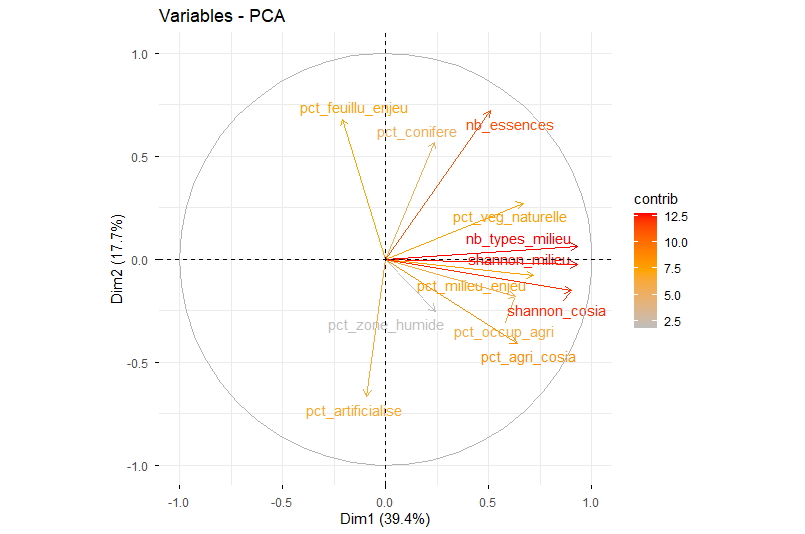
\includegraphics[width=0.9\textwidth]{acp final.png}
  \caption{Cercle des corrélations -- ACP finale CarHAB + BD Forêt + COSIA}
\end{figure}

\subsubsection*{Comment lire ce cercle}

Chaque flèche représente une variable. La \textbf{longueur} indique la qualité de représentation sur ces deux axes -- une flèche longue (proche du bord) signifie que la variable est bien capturée par Dim.1 et Dim.2. \textbf{L'angle} entre deux flèches indique la corrélation : flèches parallèles = corrélées positivement, flèches opposées = corrélées négativement, flèches perpendiculaires = indépendantes.

\begin{tcolorbox}[infobox]
  \textbf{Note :} \texttt{pct\_zone\_humide} présente une flèche courte car elle vit principalement sur Dim.3 (non affiché sur ce cercle). Elle contribue au score final mais est mal représentée sur ce plan Dim.1/Dim.2.
\end{tcolorbox}

\vspace{0.4cm}
\subsubsection*{Les trois axes}

\begin{tabularx}{\textwidth}{L{1.5cm} L{1.8cm} L{5cm} X}
  \toprule
  \rowcolor{vert!85}
  \textcolor{white}{\textbf{Axe}} &
  \textcolor{white}{\textbf{Variance}} &
  \textcolor{white}{\textbf{Variables dominantes}} &
  \textcolor{white}{\textbf{Interprétation}} \\
  \midrule
  \rowcolor{vertclair}
  Dim.1 & 39,4\% &
    nb\_types\_milieu (18,4\%), shannon\_milieu (18,2\%), shannon\_cosia (17,2\%) &
    Diversité et naturalité globale -- \textbf{axe principal} \\
  Dim.2 & 17,7\% &
    nb\_essences (24,4\%), pct\_feuillu\_enjeu (21,7\%), pct\_artificialise (21,0\%) &
    Qualité forestière vs artificialisation \\
  \rowcolor{vertclair}
  Dim.3 & $\sim$10,0\% &
    pct\_occup\_agri (29,8\%), pct\_zone\_humide (21,2\%) &
    Zones humides vs pression agricole \\
  \textbf{Total} & \textbf{57,1\%} & --- &
    Plus de la moitié de la variance totale capturée \\
  \bottomrule
\end{tabularx}

% ═══════════════════════════════════════════════
\section{Construction du Score}

\subsection{Orientation des axes}

Avant de combiner les axes, chaque axe est vérifié pour s'assurer que la direction positive correspond à un fort potentiel écologique :

\begin{tabularx}{\textwidth}{L{1.5cm} L{1.8cm} X}
  \toprule
  \rowcolor{vert!85}
  \textcolor{white}{\textbf{Axe}} &
  \textcolor{white}{\textbf{Inversion ?}} &
  \textcolor{white}{\textbf{Justification}} \\
  \midrule
  \rowcolor{vertclair}
  Dim.1 & Non &
    \texttt{shannon} (+0,93), \texttt{nb\_types} (+0,93), \texttt{shannon\_cosia} (+0,90) tous positifs \\
  Dim.2 & Oui (signe $-$) &
    \texttt{pct\_artificialise} $= -0{,}67$ : sans inversion un IRIS urbain aurait une coordonnée négative qui le pénaliserait dans le mauvais sens \\
  \rowcolor{vertclair}
  Dim.3 & Non &
    \texttt{pct\_zone\_humide} $= +0{,}54$ (positif), \texttt{pct\_occup\_agri} $= -0{,}64$ (négatif) \\
  \bottomrule
\end{tabularx}

\subsection{Formule du score brut}

\begin{lstlisting}
# Variances expliquees des 3 premiers axes
variances_final <- res_pca_final$eig[1:3, "percentage of variance"]
# => c(39.4, 17.7, 10.0)

# Coordonnees des IRIS sur les axes
coords_final <- as.data.frame(res_pca_final$ind$coord)

# Matrice : Dim.2 inversee (signe moins)
score_matrix <- cbind(
   coords_final$Dim.1,   # naturalite/diversite       -- non inverse
  -coords_final$Dim.2,   # foret vs artificialisation -- INVERSE
   coords_final$Dim.3    # zones humides vs agri      -- non inverse
)

# Produit matriciel : somme ponderee / variance cumulee
df_final$score_brut <- as.vector(
  score_matrix %*% variances_final / sum(variances_final)
)
\end{lstlisting}

Le produit matriciel calcule pour chaque IRIS :

\begin{equation}
  \text{Score brut} = \frac{\text{Dim.1} \times 39{,}4 + (-\text{Dim.2}) \times 17{,}7 + \text{Dim.3} \times 10{,}0}{67{,}1}
\end{equation}

\subsection{Normalisation 0--100 et rôle du min/max}

\begin{lstlisting}
df_final$score_biodiv_final <- with(df_final,
  (score_brut - min(score_brut)) / (max(score_brut) - min(score_brut)) * 100
)
\end{lstlisting}

\begin{equation}
  \text{Score final} = \frac{\text{Score brut} - \min(\text{Score brut})}{\max(\text{Score brut}) - \min(\text{Score brut})} \times 100
\end{equation}

\subsubsection*{Rôle du minimum}

$\min(\text{Score brut})$ est la valeur du score brut de l'\textbf{IRIS le moins écologiquement riche} du territoire -- celui qui combine le moins de milieux naturels, le plus de pression agricole et le plus d'artificialisation. En soustrayant ce minimum à tous les scores, on ramène cet IRIS à exactement 0. Tous les autres IRIS ont désormais un score positif proportionnel à leur écart avec le pire IRIS.

\subsubsection*{Rôle du maximum}

$\max(\text{Score brut}) - \min(\text{Score brut})$ est l'\textbf{étendue totale} des scores bruts -- la distance entre le pire et le meilleur IRIS du territoire. En divisant par cette étendue, on compresse toute la variabilité dans un intervalle $[0, 1]$, puis la multiplication par 100 donne l'échelle $[0, 100]$.

\subsubsection*{Exemple numérique}

Si les scores bruts vont de $-3{,}2$ (pire IRIS, vallée du Rhône) à $+4{,}8$ (meilleur IRIS, massif naturel), l'étendue est $4{,}8 - (-3{,}2) = 8{,}0$ :

\vspace{0.3cm}
\begin{tabularx}{\textwidth}{L{2.5cm} L{1.8cm} X L{2cm}}
  \toprule
  \rowcolor{vert!85}
  \textcolor{white}{\textbf{IRIS}} &
  \textcolor{white}{\textbf{Score brut}} &
  \textcolor{white}{\textbf{Calcul}} &
  \textcolor{white}{\textbf{Score final}} \\
  \midrule
  \rowcolor{vertclair}
  Pire IRIS & $-3{,}2$ & $\frac{-3{,}2 - (-3{,}2)}{8{,}0} \times 100 = \frac{0}{8} \times 100$ & \textbf{0} \\
  IRIS médian & $+0{,}8$ & $\frac{0{,}8 - (-3{,}2)}{8{,}0} \times 100 = \frac{4{,}0}{8} \times 100$ & \textbf{50} \\
  \rowcolor{vertclair}
  Meilleur IRIS & $+4{,}8$ & $\frac{4{,}8 - (-3{,}2)}{8{,}0} \times 100 = \frac{8{,}0}{8} \times 100$ & \textbf{100} \\
  \bottomrule
\end{tabularx}

\vspace{0.4cm}
\begin{tcolorbox}[infobox]
  \textbf{Conséquence importante :} le score 0 et le score 100 sont des valeurs \textbf{relatives au territoire du SCoT}. Le score 100 signifie ``l'IRIS le plus riche de ce territoire'' et non ``biodiversité parfaite''. Ce score ne peut pas être comparé directement avec un autre territoire sans recalcul complet sur la base fusionnée.
\end{tcolorbox}

% ═══════════════════════════════════════════════
\section{Validations du Score}

\subsection{Test de sensibilité des pondérations}

Les poids utilisés (variances expliquées par l'ACP) sont justifiés mathématiquement mais ne sont pas le seul choix possible. Trois scénarios ont été testés :

\vspace{0.3cm}
\begin{tabularx}{\textwidth}{L{3.5cm} L{4cm} X}
  \toprule
  \rowcolor{vert!85}
  \textcolor{white}{\textbf{Scénario}} &
  \textcolor{white}{\textbf{Poids Dim.1 / Dim.2 / Dim.3}} &
  \textcolor{white}{\textbf{Corrélation avec score ACP}} \\
  \midrule
  \rowcolor{vertclair}
  ACP -- retenu & 39,4\% / 17,7\% / 10,0\% & 1,000 (référence) \\
  Poids égaux & 33\% / 33\% / 33\% & 0,918 \\
  \rowcolor{vertclair}
  Dim.1 ultra-dominante & 60\% / 25\% / 15\% & 0,9998 \\
  \bottomrule
\end{tabularx}

\vspace{0.3cm}
Toutes les corrélations dépassent \textbf{0,90} -- seuil admis pour la robustesse d'un score composite. Le classement des IRIS est stable quel que soit le schéma de pondération.

\subsection{Contribution de chaque source}

\begin{tabularx}{\textwidth}{L{4.5cm} L{1.8cm} X}
  \toprule
  \rowcolor{vert!85}
  \textcolor{white}{\textbf{Comparaison}} &
  \textcolor{white}{\textbf{Corrélation}} &
  \textcolor{white}{\textbf{Interprétation}} \\
  \midrule
  \rowcolor{vertclair}
  Score CarHAB seul vs Score final & 0,95 & CarHAB est la source dominante \\
  Score COSIA seul vs Score final & 0,94 & COSIA apporte une information quasi équivalente à CarHAB \\
  \rowcolor{vertclair}
  Score BD Forêt seul vs Score final & 0,09 & BD Forêt déjà capturée par CarHAB et COSIA -- apport qualitatif sur Dim.2 \\
  CarHAB vs COSIA & 0,87 & Les deux sources principales sont très cohérentes entre elles \\
  \bottomrule
\end{tabularx}

% ═══════════════════════════════════════════════
\section{Cartographie et Résultats}

\subsection{Distribution du score}

\begin{tabularx}{\textwidth}{L{2.5cm} L{2cm} X}
  \toprule
  \rowcolor{vert!85}
  \textcolor{white}{\textbf{Statistique}} &
  \textcolor{white}{\textbf{Valeur}} &
  \textcolor{white}{\textbf{Interprétation}} \\
  \midrule
  \rowcolor{vertclair}
  Minimum & 0 & IRIS de référence le moins riche -- vallée du Rhône \\
  1\textsuperscript{er} quartile & $\sim$17 & 25\% des IRIS ont un score inférieur à 17 \\
  \rowcolor{vertclair}
  Médiane & $\sim$37 & IRIS médian du territoire \\
  Moyenne & $\sim$35 & Légèrement inférieure à la médiane -- asymétrie vers le bas \\
  \rowcolor{vertclair}
  3\textsuperscript{e} quartile & $\sim$49 & 75\% des IRIS ont un score inférieur à 49 \\
  Maximum & 100 & IRIS de référence le plus riche -- massifs naturels \\
  \bottomrule
\end{tabularx}

\vspace{0.3cm}
\textbf{Couverture :} 281 IRIS, 0 donnée manquante. La couverture complète est obtenue grâce à COSIA qui couvre l'intégralité du territoire.

\subsection{Carte du score de potentiel écologique}
\begin{figure}[H]
  \centering
  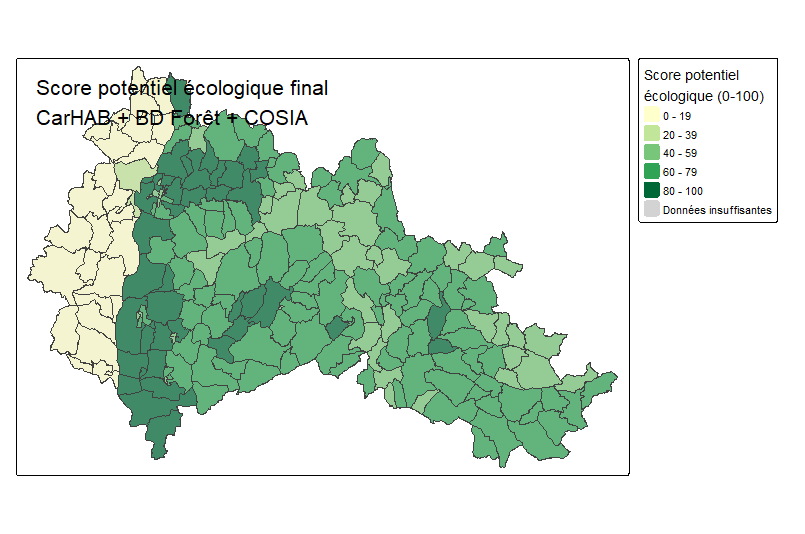
\includegraphics[width=0.85\textwidth]{score final.png}
  \caption{Score de potentiel écologique par IRIS (0--100) -- CarHAB + BD Forêt + COSIA -- Mars 2026}
\end{figure}

\subsection{Interprétation spatiale}

\begin{itemize}[leftmargin=1.5cm]
  \item \textbf{Zones foncées (80--100) :} massifs naturels du centre et du sud -- forte couverture en feuillus, milieux ouverts diversifiés, faible artificialisation. Quelques IRIS isolés à fort score à l'est correspondent probablement à des vallées encaissées avec zones humides et ripisylves.
  \item \textbf{Zones moyennes (40--60) :} espaces de transition -- diversité de milieux correcte mais pression agricole modérée.
  \item \textbf{Zones claires (0--20) :} vallée du Rhône à l'ouest et zones périurbaines -- forte artificialisation, prédominance des cultures et de la vigne.
  \item \textbf{Continuité spatiale :} le score varie progressivement sans ruptures artificielles, ce qui valide la cohérence méthodologique.
\end{itemize}

% ═══════════════════════════════════════════════
\section{Limites et Perspectives}

\subsection{Limites}

\begin{itemize}[leftmargin=1.5cm]
  \item \textbf{Relativité du score :} le score 100 signifie ``le meilleur IRIS du territoire'' et non une valeur absolue de biodiversité. Non comparable entre territoires sans recalcul.
  \item \textbf{Absence de connectivité :} un IRIS à fort potentiel isolé de zones naturelles voisines a une valeur écologique moindre qu'un IRIS équivalent en continuité. La connectivité n'est pas encore intégrée.
  \item \textbf{BD Forêt datée de 2014 :} les dynamiques forestières récentes (incendies, coupes) ne sont pas prises en compte.
  \item \textbf{Zones humides sous-représentées dans l'ACP :} rares sur le territoire, leur variance spatiale est faible même si leur valeur écologique est forte.
\end{itemize}
%======================================================

\chapter*{Conclusion}

Le projet EcoLab apporte une réponse technique innovante et exhaustive pour l'évaluation de l'artificialisation et du potentiel écologique sur le territoire du SCOT Drôme-Ardèche. En combinant des approches méthodologiques complémentaires, ce rapport démontre la faisabilité et la pertinence d'un outil d'aide à la décision à très haute résolution :

\begin{itemize}
    \item \textbf{Une modélisation hybride à l'échelle parcellaire :} L'intégration de l'Intelligence Artificielle (modélisation thématique BERTopic et scoring LLM via Mistral) à l'analyse spatiale (croisements avec la BD TOPO et COSIA) permet de capturer avec finesse le signal environnemental local. Ces traitements aboutissent à la création d'une cartographie web interactive performante, facilitant l'exploration des enjeux de chaque parcelle.
    \item \textbf{Un score statistique composite à l'échelle de l'IRIS :} Grâce à l'Analyse en Composantes Principales (ACP) exploitant les données officielles (CarHAB, BD Forêt, COSIA), 12 indicateurs ont été synthétisés pour créer un score robuste de potentiel écologique, échelonné de 0 à 100.
\end{itemize}

Ces travaux se matérialisent par des livrables concrets, notamment des bases de données optimisées (GeoPackage) et des styles automatisés pour QGIS. Ils offrent aux décideurs une base reproductible pour identifier les zones à fort potentiel, orienter les inventaires naturalistes et argumenter les zonages de protection dans le cadre des révisions du SCOT et des PLUi.

Toutefois, pour consolider et faire évoluer ce dispositif, les prochaines itérations devront prendre en compte certaines limites inhérentes aux données et aux modèles actuels. Il s'agira notamment :

\begin{itemize}
    \item D'intégrer des métriques de connectivité écologique, essentielles pour évaluer la valeur réelle d'une zone au sein de son réseau.
    \item De s'appuyer sur des données forestières plus récentes pour capturer les dynamiques actuelles (incendies, coupes), la BD Forêt utilisée datant de 2014.
    \item De mieux pondérer la valeur des zones humides, dont l'importance écologique est majeure malgré leur sous-représentation mathématique dans l'ACP actuelle.
\end{itemize}

\end{document}
